\documentclass[a4paper, 14pt]{extarticle}
\usepackage{graphicx}
\usepackage[T2A]{fontenc}
\usepackage[utf8]{inputenc}
\usepackage[russian]{babel}
\usepackage{setspace,amsmath}
\usepackage{hyperref}
\usepackage{amsfonts}
\usepackage[left=20mm, top=15mm, right=15mm, bottom=15mm, nohead, footskip=10mm]{geometry} % Настройки полей документа

\graphicspath{ {./images/} }

\makeatletter
\newcommand{\verbatimfont}[1]{\renewcommand{\verbatim@font}{\ttfamily#1}}
\makeatother

\begin{document} % Начало документа

% Начало титульного листа
\begin{center}
    \normalsize{\textbf{МИНИСТЕРСТВО ОБРАЗОВАНИЯ РЕСПУБЛИКИ БЕЛАРУСЬ}}\\
    \hfill \break
    \normalsize{\textbf{БЕЛОРУССКИЙ ГОСУДАРСТВЕННЫЙ УНИВЕРСИТЕТ}}\\
    \hfill \break
    \small{\textbf{ФАКУЛЬТЕТ ПРИКЛАДНОЙ МАТЕМАТИКИ И ИНФОРМАТИКИ}}\\
    \hfill \break
    \large{Кафедра математического моделирования и анализа данных}\\
    \vspace{40mm}
    \normalsize{БОЛТАЧ}\\
    \hfill \break
    \normalsize{Антон Юрьевич}\\
    \hfill \break
    \normalsize{\textbf{Криптография на основе функций хэширования:\\ подписи без состояния}}\\
    \hfill \break
    \normalsize{Дипломная работа}\\
    \hfill \break
\end{center}

\begin{flushright}
    \vspace{20mm}
    Научный руководитель:\\
    кандидат физ.-мат. наук,\\
    Агиевич Сергей Валерьевич\\
\end{flushright}

\begin{flushleft}
    \vspace{20mm}
    Допущен к защите\\
    “\underline{\hspace{8mm}}” \underline{\hspace{4cm}}2020 г.\\
    Зав. кафедрой ММАД\\
    кандидат физ.-мат. наук, доцент И.А. Бодягин\\
\end{flushleft}

\vfill
\begin{center}
    Минск, 2020 г.
\end{center}
\thispagestyle{empty} % Выключаем отображение номера для этой страницы
    
% Конец титульного листа

\newpage

% Содержание
\tableofcontents
\newpage

% Реферат
\section*{\centerline{РЕФЕРАТ}}
\addcontentsline{toc}{section}{\protect\numberline{}РЕФЕРАТ}
\centerline{Дипломная работа, 34 с., 6 рис., 1 табл., 7 источников, 1 прил.}

\textbf{\newline Ключевые слова:} ЭЦП, ОДНОРАЗОВЫЕ ПОДПИСИ, ДЕРЕВЬЯ МЕРКЛЯ, МНОГОРАЗОВЫЕ ПОДПИСИ, ПОДПИСИ БЕЗ СОСТОЯНИЯ, БЛОКЧЕЙН BITSHARES.

\textbf{\newline Объект исследования} --- ЭЦП на основе функций хэширования: подписи без состояния.

\textbf{\newline Цель работы} --- изучить возможность использования на практике систем ЭЦП на основе функций хэширования без состояния.

\textbf{\newline Результаты работы} --- проведён сравнительный анализ систем ЭЦП на основе функций хэширования без состояния; разработаны программные реализации систем SPHINCS, $\text{SPHINCS}^+$, Gravity-SPHINCS; программные реализации интегрированы в блокчейн-систему Bitshares.

\newpage

\section*{\centerline{РЭФЕРАТ}}
\centerline{Дыпломная работа, 34 с., 6 мал., 1 табл., 7 крыніц, 1 прыкл.}

\textbf{\newline Ключавыя словы:} ЭЦП, АДНАРАЗОВЫЯ ПОДПІСЫ, ДРЭВЫ МЕРКЛЯ, ШМАТРАЗОВЫЯ ПОДПИСИ, ПОДПІСЫ БЕЗ СТАНУ, БЛОКЧЕЙН BIT-\\SHARES.

\textbf{\newline Аб’ект даследавання} --- ЭЦП на аснове функцый хэшавання: подпісы без стану.

\textbf{\newline Мэта работы} --- даследаваць магчымасць выкарыстання на практыцы сістэм ЭЦП на аснове функцый хэшавання без стану.

\textbf{\newline Вынiк работы} --- праведзены параўнальны аналіз сістэм ЭЦП на аснове функцый хэшавання без стану; распрацаваны праграмныя рэалізацыі сістэм SPHINCS, $\text{SPHINCS}^+$, Gravity-SPHINCS; праграмныя рэалізацыі інтэграваны ў блокчейн-сістэму Bitshares.

\newpage

\section*{\centerline{ABSTRACT}}
\centerline{Diploma work, 34 p., 6 pic., 1 tab., 7 sources, 1 app.}

\textbf{\newline Keywords:} DIGITAL SIGNATURE, ONE-TIME SIGNATURE, MERKLE \\SIGNATURE SCHEME, FEW-TIME SIGNATURES, STATELESS SIGNATURES, BLOCKCHAIN BITSHARES.

\textbf{\newline Object of research} --- Hash based digital signatures: stateless.

\textbf{\newline Purpose of work} --- research hash-based stateless digital signature algorithms in practice.

\textbf{\newline Results of work} --- a comparative analysis of hash-based stateless digital signature algorithms; development SPHINCS, $\text{SPHINCS}^+$, Gravity-SPHINCS systems; integrated into the Bitshares blockchain system.

\newpage

% Введение
% Концепции Hash-based crypto
\section*{Введение}
\addcontentsline{toc}{section}{\protect\numberline{}Введение}
Цифровые подписи широко используются в Интернете, в частности, для аутентификации, проверки целостности и отказа от авторства. Алгоритмы цифровой подписи, наиболее часто используемые на практике --- RSA, DSA и ECDSA, основаны на допущениях сложности задач теории чисел, а именно факторизации целых чисел и дискретного логарифмирования. В 1994 году Питер Шор показал, что эти вычислительные задачи могут стать решены эффективно при наличии квантовых компьютеров. Квантовые компьютеры могут решить их за полиномиальное время, ставя под угрозу безопасность схем цифровой подписи, используемых сегодня. Хотя квантовые компьютеры еще не могут решать практические задачи, их развитие происходит быстрыми темпами и поэтому представляет собой реальную угрозу в течение следующих десятилетий. К счастью, постквантовая криптография предоставляет множество квантовостойких альтернатив классическим схемам цифровой подписи.

Подписи на основе функций хэширования, являются одной из наиболее многообещающих из этих альтернатив. Мы говорим, о сравнительно новой криптографической платформе HBC (Hash-Based Cryptography), которая представляет собой криптографические примитивы, основанные на безопасности хэш-функции. Это одна из популярных платформ конкурса NIST PostQuatum Cry-pto. В первом раунде было более 70-и заявок алгоритмов из класса HBC, из них 27 прошли во второй раунд.

\textbf{Цель дипломной работы:} изучение системы ЭЦП без состояния SPHINCS, $\text{SPHINCS}^+$, Gravity-SPHINCS. Реализовать системы ЭЦП без состояния на языке Python. Интегрировать в блокчейн-систему и провести оценку быстродействия разработанных реализаций.

\textbf{Задачи дипломной работы:} исходя из цели можно поставить следующие задачи.

\begin{enumerate}
    \item Изучение публикаций по основам HBC (Hash-Based Cryptography).
    \item Разобрать устройство систем SPHINCS, $\text{SPHINCS}^+$, Gravity-SPHINCS.
    \item Реализовать систему ЭЦП без состояния программно и интегрировать программную реализацию в блокчейн-систему.
    \item Оценить быстродействие разработанных реализаций для подписи транзакций в блокчейн-системе.
\end{enumerate}

\newpage

% Классификация подписей на основе функций хэширования
\section{Подписи на основе функций хэширования}
\subsection{Введение}
Пусть $H : \{0, 1\}^{*} \rightarrow \{0, 1\}^{*}$ криптографическая хэш-функция.

Исходное сообщение $m$, для которого вычислено хэш-значение, называется прообразом хэш-функции.

К криптографическим хэш-функциям предъявляются следующие требования:

\begin{enumerate}
    \item Сопротивление поиску первого прообраза: при наличии хэша $h$ должно быть \emph{трудно} найти какое-либо сообщение $m$, такое что $h=H(m)$.
    \item Сопротивление поиску второго прообраза: при наличии сообщения $m_{1}$, должно быть \emph{трудно} найти другое сообщение $m_{2}$ ($m_{1} \neq m_{2}$) такое, что $H(m_{1})\ =\ H(m_{2})$.
    \item Стойкость к коллизиям.

    Коллизией для хэш-функции называется такая пара значений $m$ и $m^{'}$, $m \neq m^{'}$, для которой $H(m)\ =\ H(m^{'})$.

    Стойкость хэш-функции к коллизиям означает, что нет эффективного полиномиального алгоритма, позволяющего находить коллизии.
\end{enumerate}

Данные свойства не являются независимыми:

\begin{itemize}
    \item Функция, нестойкая к восстановлению второго прообраза, нестойка к коллизиям; обратное неверно.
    \item Функция устойчивая к коллизиям, устойчива к нахождению второго прообраза.
    \item Устойчивая к коллизиям хэш-функция не обязательно является односторонней.
\end{itemize}

В HBC (Hash-Based Cryptography) используются хэш-функции, для которых важна только задача сопротивления поиска первого прообраза. Основная идея HBC в том, что безопасность подписи гарантируется выбором безопасной хэш-функции. Покажем это на примере подписи Лампорта, но сперва введем формальное определение ЭЦП.

Формально схема цифровой подписи представляет собой тройку алгоритмов (Gen, Sign, Verify).

Схема одноразовой подписи Лампорта на примере хэш-функции SHA-256:

\begin{itemize}
    \item Алгоритм генерации ключей Gen:

    \begin{itemize}
        \item Вход: $1^{n}$, где $n$ --- параметр безопасности.
        \item Выход: Открытый ключ ($pk$) и соответствующий личный ключ ($sk$).
    \end{itemize}

    На входе параметр $n$, который определяет надежность системы ЭЦП. С ростом $n$, как правило растут длины $pk$ и $sk$, а также увеличивается трудоёмкость алгоритма.

    Личный ключ $sk$ представляет собой таблицу, содержащую $2\ *\ 256\ =\ 512$ случайных строк, как показано ниже:

    \begin{center}
        \begin{tabular}{ |c|c|c|c|c|c| } 
         \hline
         $sk^{1}_{0}$ & $sk^{2}_{0}$ & \hspace{3mm} & ... & \hspace{3mm} & $sk^{256}_{0}$ \\ 
         \hline
         $sk^{1}_{1}$ & $sk^{2}_{1}$ & \hspace{3mm} & ... & \hspace{3mm} & $sk^{256}_{1}$ \\ 
         \hline
        \end{tabular}
    \end{center}

    Пусть $H$ это наша хэш-функция SHA-256. Тогда для получения открытого ключа $pk$ применяем хэш-функцию $H$ ко всем строкам личного ключа $sk$ из таблицы выше:
    \[pk_{1}=H(sk^{1}_{0}), pk_{2}=H(sk^{1}_{1}), ..., pk_{512}=H(sk^{256}_{1})\text{.}\]

    \item Алгоритм подписи Sign:

    \begin{itemize}
        \item Вход: Cообщение $m$ и личный ключ $sk$.
        \item Выход: Подпись $\sigma$.
    \end{itemize}

    Применим хэш-функцию $H$ и получим хэш-значение сообщения $H(m)=m_{1}m_{2}...m_{256}$. Далее, чтобы получить подпись $\sigma$ придерживаемся следующего условия:

    \begin{enumerate}
        \item Если $m_{i}\ =\ 0$, выбираем $sk^{i}_{0}$.
        \item Если $m_{i}\ =\ 1$, выбираем $sk^{i}_{1}$.
        
        Где $i \in \{1, 256\}$.
    \end{enumerate}

    Получаем $\sigma = sk^{1}_{m_{1}}, sk^{2}_{m_{2}}, ..., sk^{256}_{m_{256}}$

    \item Алгоритм проверки подписи Verify:

    \begin{itemize}
        \item Вход: Открытый ключ $pk$, сообщение $m$ и подпись $\sigma$.
        \item Выход: 1 (подпись корректна) или 0 (нет).
    \end{itemize}

    Проверяем, что $H(sk^{i}_{m_{i}}) = pk^{i}_{m_{i}}, \forall i \in \{1, 256\}$.
\end{itemize}

\newpage

\subsection{Классификация}
В нашей работе мы приводим классификацию систем ЭЦП на основе функций хэширования. Исследуем системы с состоянием (Stateful), при этом выделяем системы без состояния (Stateless) как самую безопасную альтерантиву.\newline

В основном подписи на основе функций хэширования подразделяются на:

\begin{enumerate}
    \item Подписи с состоянием Stateful:

    В этих системах алгоритм Gen, кроме $sk$ (личного ключа) возвращает $st$ (состояние), и $st$ является и дополнительным входом, и дополнительным выходом алгоритма Sign.

    Подписи с состоянием разделяются на:

    \begin{enumerate}
        \item Одноразовые подписи OTS (One-Time Signature).
        \item Многоразовые подписи FTS (Few-Time Signature).
    \end{enumerate}

    \item Подписи без состояния Stateless.

    В подписях с состоянием возникают проблемы с их использованием на практике, так как нам необходимо хранить состояние. Это не соответсвует стандарту APIs (Application Programming Interface), это даже не соответствует стандартному определению подписей в криптографии. Если обновление состояния не удаётся (например, если ключ скопирован с одного устрайства на другое, или скопирован в резервную копию и позже восстановлен), то безопасность нарушается.

    Поэтому выделям системы ЭЦП без состояния, такие как \nameref{gravity-sphincs}, \nameref{sec_sphincs}, \nameref{sec_sphincsplus}.
\end{enumerate}

\begin{figure}[h]
    \centering
    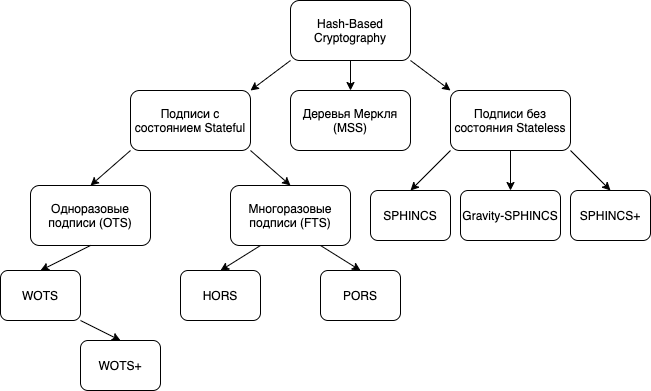
\includegraphics[scale=0.72]{HBC_structure.png}
    \caption{Криптография на основе функций хэширования}
    \label{fig:hbc_structure}
\end{figure}

% Одноразовые подписи
\subsection{Одноразовые подписи}
\label{ots}
Одноразовые подписи $OTS$ (One-Time Signature) называются одноразовыми, поскольку безопасность сообщения гарантируется только при однократном использовании ключей. Однако, преимущества OTS заключаются в том, что они могут быть построены из любой односторонней функции, а алгоритмы подписи и проверки очень быстры в вычислениях (по сравнению с другими подписями на основе функций хэширования).
\subsubsection{Одноразовая подпись Винтерница}
WOTS (Winternitz One-Time Signature) \cite{wots} --- основная идея заключается в итеративном применении хэш-функции, в то время как количество итераций зависит от сообщения, которое должно быть подписано. WOTS использует хэш функцию $F : \{0, 1\}^{n} \rightarrow \{0, 1\}^{n}$. Она параметризуется длиной сообщения $m$ и параметром $w \in \mathbb{N}$, $w > 1$, который определяет компромисс между временем и памятью.

Теперь опишем три алгоритма подписи:

\begin{itemize}
    \item Алгоритм генерации ключей Gen:

    \begin{itemize}
        \item Вход: $1^{n}$, где $n$ --- параметр безопасности.
        \item Выход: Открытый ключ ($pk$) и соответствующий личный ключ ($sk$).
    \end{itemize}

    Сперва выбираем параметр $w \in \mathbb{N}$, $w > 1$.
    Личный ключ состоит из $l$ битовых блоков длиной $n$, выбранных равномерно со случайным распределением, 
    \[sk = (sk_{1}, ..., sk_{l}) \stackrel{\$}\leftarrow \{0, 1\}^{(n,l)}\text{,}\]

    где $l$ вычисляется как:
    \[ l_{1} = \Bigg \lceil \frac{m}{log_{2}(w)} \Bigg \rceil, l_{2} = \Bigg \lfloor \frac{log_{2}(l_{1}(w - 1))}{log_{2}(w)} \Bigg \rfloor + 1, l = l_{1} + l_{2}. \]

    Открытый ключ проверки $pk$ вычисляется как:
    \[ pk = (pk_{1}, ..., pk_{l}) = (F^{w - 1}_{sk_{1}}(x), ..., F^{w - 1}_{sk_{l}}(x)) \]

    \item Алгоритм подписи Sign:

    \begin{itemize}
        \item Вход: Cообщение $M^{*}$ и личный ключ $sk$.
        \item Выход: Подпись $\sigma$.
    \end{itemize}

    Сообщение $M^{*}$ длины $m$ и личного ключа подписи $sk$, алгоритм подписи сначала вычисляет базовое $w$ представление
    \[M^{*}: M^{*} = (M^{*}_{1}, ..., M^{*}_{l_{1}}), M^{*}_{i} \in \{0, ..., w - 1\}\]

    и вычисляет его базовое $w$ представление $C = (C_{1}, ..., C_{l_2})$. Длина базового $w$ представления $C$ не более $l_{2}$, так как $C \leq l_{1}(w - 1)$. Мы задаем $B = (B_{1}, ..., B_{l}) = M^{*} || C$. Подпись вычисляется как
    \[ \sigma = (\sigma_{1}, ..., \sigma_{l}) = (F^{B_1}(sk_{1}), ..., F^{B_l}(sk_{l})) \]

    \item Алгоритм проверки подписи Verify:

    \begin{itemize}
        \item Вход: Открытый ключ $pk$, сообщение $M^{*}$ и подпись $\sigma$.
        \item Выход: 1 (подпись корректна) или 0 (нет).
    \end{itemize}

    Сообщение $M^{*}$ длины $m$, подпись $\sigma$ и открытый ключ проверки $pk$, алгоритм проверки сначала вычисляет $B_{i}$, $ 1 \leq i \leq l$, как описано выше. Затем он выполняет следующее сравнение:
    \[ pk = (pk_{1}, ..., pk_{l}) \stackrel{?}= (F^{w - 1 - B_{1}}(\sigma_{1}), ..., (F^{w - 1 - B_{l}}(\sigma_{l})) \]

    Если сравнение выполняется, возвращаем 1 или 0 в ином случае.
\end{itemize}

Схема подписи без контрольной суммы может быть просто нарушена: после того, как подписавшая сторона выдаст действительную подпись для какого-либо сообщения, любой может легко создать подпись для сообщения $M^{'} = (M^{'}_1, ..., M^{'}_{l_{1}})$, если $M^{'}_{i} \leq M^{*}_{i}$ для всех $i$.

Идея исправления проблемы заключается в следующем, помимо подписания сообщения, мы так же должны подписать некоторую дополнительную строку, которую назовем контрольной суммой и вычислим следующем образом:
\[ C = \sum^{l_{1}}_{i = 1}(w - 1 - M^{*}_{i}) \]

\subsubsection{Дополненная подпись Винтерница}
Введем вариант подписи Винтерница $\text{WOTS}^{+}$ ($\text{Winternitz One-Time Signature}^+$) \cite{wotsplus}, который позволяет уменьшить размер подписи и достигает более высокого уровня безопасности. Как и все варианты $W\-OTS$, $W\-OTS^{+}$ параметризуется параметром безопасности $n \in \mathbb{N}$, длиной сообщения $m$ и параметром $w \in \mathbb{N}$, $w > 1$, который определяет компромисс между временем и памятью. Последние два параметра используются для вычисления
\[ l_{1} = \Bigg \lceil \frac{m}{log_{2}(w)} \Bigg \rceil, l_{2} = \Bigg \lfloor \frac{log_{2}(l_{1}(w - 1))}{log_{2}(w)} \Bigg \rfloor + 1, l = l_{1} + l_{2}. \]

Кроме того, $W\-OTS^{+}$ использует семейство функций $F_{n} : \{f_{k} : \{0, 1\}^{n} \rightarrow \{0, 1\}^{n}|k \in K_{n}\}$ с ключевым пространством $K_{n}$. Можно предположить как о криптографическом семействе хэш-функций, которое не сжимается. Используя $F_{n}$, мы определяем следующую функцию.

$c^{i}_{k}(x, r):$ На входе значения $x \in \{0, 1\}^{n}$, счетчика итераций $i \in \mathbb{N}$, ключа $k \in K$ и элементы случайности $r = (r_{1}, ..., r_{j}) \in \{0, 1\}^{n \times j}$ при $j \geq i$, функция работает следующим образом:

\begin{itemize}
    \item В случае $i = 0$, $c^{i}_{k}(x, r)$ возвращает $x(c^{0}_{k}(x, r) = x)$.
    \item Для $i > 0$ мы определяем $c^{i}_{k}(x, r)$ рекурсивно как
    \[ c^{i}_{k}(x, r) = f_{k}(c^{i - 1}_{k}(x, r) \oplus r_{i}) ,\]
\end{itemize}

То есть в каждом раунде функция сначала принимает побитовый $xor$ промежуточного значения и битовую маску $r$, затем оценивает $f_{k}$ на результат. Мы пишем $r_{a,b}$ для подмножества $r_{a}, ..., r_{b}$ как $r$. В случае $b < a$ мы определяем $r_{a,b}$ как пустую строку. Будем считать, что параметры $m$, $w$ и семейство функций $F_{n}$ общеизвестны.

Теперь опишем три алгоритма подписи $W\-OTS^{+}$:

\begin{itemize}
    \item Алгоритм генерации ключа Gen:

    \begin{itemize}
        \item Вход: $1^{n}$, где $n$ --- параметр безопасности.
        \item Выход: Открытый ключ ($pk$) и соответствующий личный ключ ($sk$).
    \end{itemize}

    При вводе параметра безопасности $n$ унарно, алгоритм генерации ключа выбирает $l + w - 1$ $n$-бит равномерно случайным образом. Личный ключ $sk = (sk_{1}, ..., sk_{l})$ состоит из первых $l$ случайных битовых блоков. Оставшиеся $w - 1$ бит используются в качестве элементов случайности $r = (r_{1}, ..., r_{w - 1})$ для $c$. Далее, $Gen$ выбирает функцию ключа $k \stackrel{\$}\leftarrow K$ равномерно случайным образом. Открытый ключ проверки $pk$ вычисляется как
    \[ pk = (pk_{0}, pk_{1}, ..., pk_{l}) = ((r, k),c^{w - 1}_{k}(sk_{1},r), ..., c^{w - 1}_{k}(sk_{l}, r)). \]

    \item Алгоритм подписи Sign:

    \begin{itemize}
        \item Вход: Cообщение $M$ и личный ключ $sk$.
        \item Выход: Подпись $\sigma$.
    \end{itemize}

    На входе $m$ битного сообщения $M$, личного ключа подписи $sk$ и элементов случайности $r$, алгоритм подписи сначала вычисляет базовое $w$ представление $M: M = (M_{1} . . . M_{l_{1}} )$, $M_{i} \in \{0, ..., w - 1\}$. Поэтому $M$ рассматривается как двоичное представление натурального числа $x$, а затем вычисляется $w$ бинарное представление $x$. Далее вычисляем контрольную сумму:
    \[ C = \sum^{l_{1}}_{i = 1}(w - 1 - M_{i}) \]
    и его базовое $w$ представление $C = (C_{1}, ..., C_{l_{2}})$. Длина базового $w$ представления $C$ не более $l_{2}$, так как $C \leq l_{1}(w - 1)$. Мы задаем $B = (b_{1}, ..., b_{l}) = M || C$, конкатенация базовых $w$ представлений $M$ и $C$. Подпись вычисляется как
    \[ \sigma = (\sigma_{1}, ..., \sigma_{l}) = (c^{b_{1}}_{k}(sk_{1},r), ..., c^{b_{l}}_{k}(sk_{l},r)). \]

    Обратите внимание, что контрольная сумма гарантирует, что с учетом $b_{i}, 0 < i \leq l$, соответствующего одному сообщению, $b^{*}_{i}$ соответствующий любому другому сообщению включает по крайней мере один $b^{*}_{i} < b_{i}$.

    \item Алгоритм проверки подписи Verify:

    \begin{itemize}
        \item Вход: Открытый ключ $pk$, сообщение $M$ и подпись $\sigma$.
        \item Выход: 1 (подпись корректна) или 0 (нет).
    \end{itemize}

    На входе сообщение $M$ двоичной длины $m$, подпись $\sigma$ и открытый ключ $pk$. Алгоритм проверки сначала вычисляет $b_{i}, 1 \leq i \leq l$, как описано выше. Затем он выполняет следующее сравнение:
    \[ pk = (pk_{0}, pk_{1}, ..., pk_{l}) \stackrel{?}{=} ((r,k),c^{w - 1 - b_{1}}_{k}(\sigma_{1}, r_{b_{1} + 1, w - 1}, ..., c^{w - 1 - b_{l}}_{k}(\sigma_{l}, r_{b_{l} + 1, w - 1}))\]

    Если сравнение выполняется, возвращаем 1 или 0 в ином случае.
\end{itemize}

Время выполнения всех трех алгоритмов ограничено $l$ и $w$ оценками $f_{k}$. Размер подписи и личного ключа составляет $|\sigma| = |sk| = l*n$ бит. Размер открытого ключа равен $(l + w - 1)n + |k|$ бит, где $|k|$ обозначает количество бит, необходимых для представления любого элемента $K$.

% Схема подписи Меркля
\subsubsection{Схема подписи Меркля}
Первый способ создать схему многократной подписи MSS (Merkle Signature Scheme) из схемы одноразовой подписи --- использовать конструкцию, предложенную Мерклом в 1989 году. Учитывая целые числа $n$, $h$ и хэш-функцию $H$ : $\{0, 1\}^{2n} \rightarrow \{0, 1\}^{n}$, так называемое дерево Меркля представляет собой двоичное дерево высоты $h$, узлы которого помечены значением $x \in \{0, 1\}^{n}$, таким образом, что значение каждого внутреннего узла вычисляется как $x = H(y||z)$, где $y$ и $z$ --- значения левых и правых дочерних элементов.

Эта конструкция позволяет превратить схему одноразовой подписи в схему многократной подписи следующим образом. Учитывая $2^h$ экземпляров OTS, подписывающий создает дерево Меркля, каждое листовое значение которого являются открытым ключом экземпляра OTS. Общий открытый ключ --- это корневое значение (см. Рис. \ref{fig:MSS}).

\begin{figure}[h]
    \centering
    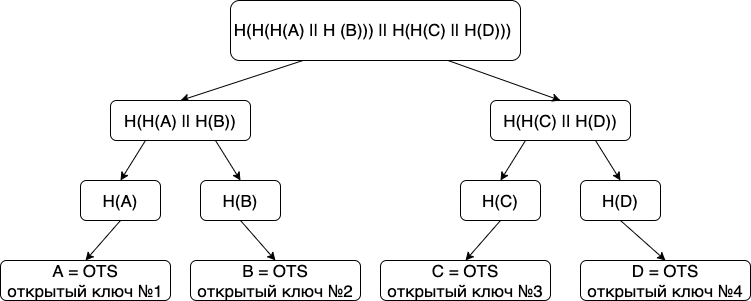
\includegraphics[scale=0.55]{MSS.png}
    \caption{Пример MSS.}
    \label{fig:MSS}
\end{figure}

Исходя из примера, чтобы подписать сообщение: используем первый открытый ключ OTS (A), а затем никогда больше не используем его, чтобы не нарушить безопасность. Затем используем открытый ключ OTS (B), затем OTS (C), и, наконец, OTS (D). Таким образом, мы можем подписать 4 сообщения в общей сложности с помощью нашего дерева. Следовательно, более большое дерево позволит нам подписывать больше сообщений.

Привлекательной идеей здесь является то, что открытый ключ состоит только из корня дерева, и каждый раз, когда мы подписываем сообщение, наша подпись состоит только из нескольких хэшей и назовем это путь аутентификации (см. Рис. \ref{fig:MSS_auth_path}).

В нашем примере подпись с первым ключом OTS (A) была бы набором элементов (1, $\sigma$, $pk$ (А), $auth$):

\begin{itemize}
    \item 1 --- это индекс листа подписи. Мы должны иметь это в виду: мы не можем повторно использовать OTS этого листа. Это делает нашу схему статичной.
    \item $\sigma$ --- это подпись OTS.
    \item $pk$ (А) --- это открытый ключ OTS.
    \item $auth$ --- это список узлов (так называемый список хэшей), который позволяет нам вычислить корень (наш основной открытый ключ).
\end{itemize}

\begin{figure}[h]
    \centering
    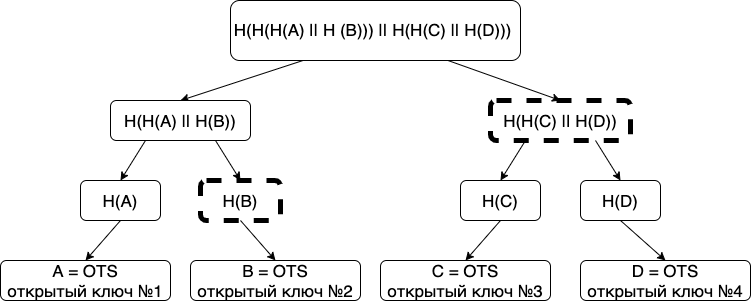
\includegraphics[scale=0.66]{MSS_auth_path.png}
    \caption{Пример MSS c выделенными блоками пути аутентификации.}
    \label{fig:MSS_auth_path}
\end{figure}

Мы видим, что с помощью нашего открытого ключа OTS и двух наших хэшей (соседние узлы всех узлов на пути от нашего подписывающего листа до корня) мы можем вычислить основной открытый ключ. И таким образом мы можем проверить, что это действительно была подпись, которая была получена от этого основного открытого ключа.

Благодаря этой схеме мы не знаем всех открытых ключей OTS для проверки основного открытого ключа. Следовательно, схема MSS экономит память и вычисления.

Время генерации ключа экспоненциально $h$, потому что на этом этапе необходимо вычислить полное дерево Меркля. Например, $h$ = 20 возможно, но может быть недостаточно для всех подписывающих. Кроме того, подписывающий должен отслеживать индексы $i$, которые уже были использованы, поэтому схема является $stateful$.

% Многоразовые подписи
\subsection{Многоразовые подписи}
\label{fts}
В то время как одноразовые подписи обеспечивают удовлетворительную криптографическую безопасность для подписания и проверки транзакций, для них характерен существенный недостаток --- их можно использовать безопасно только один раз. Поэтому существуют схемы подписи FTS (Few-Time Signature), позволяющей подписывать несколько раз одним и тем же личным ключем.
\subsubsection{HORS}
HORS (Hash to Obtain Random Subset) --- это многоразовая схема подписи. Пусть $f$ --- односторонняя функция, а $H$ --- хэш-функция, которая выводит случайный размер подмножества $\{1,2,...,t\}$, где $k$ и $t$ - параметры, влияющие на безопасность с помощью $k < t$. Параметры $k$ и $t$ также влияют на то, что длина личного ключа (и, следовательно, открытого ключа) будет $t$, в то время как подписи будут длиной $t$. Ключ подписи --- это случайный кортеж $(s_1,...,s_t)$, а открытым ключом является $(f(s_{1}),..., f(s_{t}))$.
\newline

Теперь опишем три алгоритма подписи HORS:

\begin{itemize}
    \item Алгоритм генерации ключа Gen:

    \begin{itemize}
        \item Вход: Параметры $l$, $k$, $t$.

        Шаги:
        \begin{enumerate}
            \item Генерируем $t$ случайных $l$-битовых строк $s_{1}, s_{2}, ..., s_{t}$.
            \item Пусть $v_{i} = f(s_{i})$ для $1 \leq i \leq t$.
        \end{enumerate}

        \item Выход: Открытый ключ $PK = (k, v_{1}, v_{2}, ..., v_{t})$ и личный ключ $SK = (k, s_{1}, s_{2}, ..., s_{t})$.
    \end{itemize}

    \item Алгоритм подписи Sign:

    \begin{itemize}
        \item Вход: Сообщение $m$ и личный ключ $SK = (k, s_{1}, s_{2}, ..., s_{t})$.

        Шаги:
        \begin{enumerate}
            \item Пусть $h = Hash(m)$
            \item Разбиваем $h$ на $k$ подстрок $h_{1}, h_{2}, ..., h_{k}$ длины $log_{2}t$ бит каждый.
            \item Представим каждое $h_{j}$ как целое $i_{j}$ для $1 \leq j \leq k$.
        \end{enumerate}

        \item Выход: Подпись $\sigma = (s_{i_{1}}, s_{i_{2}}, ..., s_{i_{k}})$.
    \end{itemize}

    \item Алгоритм проверки Verify:

    \begin{itemize}
        \item Вход: Сообщение $m$, подпись $\sigma = (s^{'}_{1}, s^{'}_{2}, ..., s^{'}_{k})$ и открытый ключ $PK = (k, v_{1}, v_{2}, ..., v_{t})$.

        Шаги:
        \begin{enumerate}
            \item Пусть $h = Hash(m)$
            \item Разбиваем $h$ на $k$ подстрок $h_{1}, h_{2}, ..., h_{k}$ длины $log_{2}t$ бит каждый.
            \item Представим каждое $h_{j}$ как целое $i_{j}$ для $1 \leq j \leq k$.
        \end{enumerate}

        \item Выход: Успешно, если для каждого $j$, $1 \leq j \leq k$, $f(s^{'}_{j}) = v^{i_{j}}$; Отклонено, в ином случае.
    \end{itemize}

\end{itemize}

\subsubsection{PORS}
PORS (PRNG to Obtain Random Subset, где PRNG генератор псевдослучайных чисел), где используется PRNG для получения случайного подмножества. Алгоритмы генерации ключей, подписи и проверки аналогичны HORS, но в отличии от HORS, где используется хэш-функция, задаём начальное состояние $s_{0}$, где $s_{i} \in S$ ($S$ --- это конечный набор состояний) PRNG для сообщения и запрашиваем его до тех пор, пока не получим $k$ различных индексов. Расходы в этом случае на вычисления минимальны, но значительно повышает безопасность.

\newpage

% Подписи без состояния
\section{Подписи без состояния}
\label{stateless}
\subsection{SPHINCS}
\label{sec_sphincs}
SPHINCS \cite{stateless} --- подпись, сочетающая в себе большое количество достижений в области HBC (Hash-Based Cryptography). Данная подпись обеспечивает нам самое главное избавление от состояния. Это означает, что нам больше не нужно сохранять и обновлять состояние подписи и поэтому SPHINCS называется Stateless (без состояния) подписью.
Представим основные идеи SPHINCS, описав его как комбинацию четырех типов деревьев. Ниже перечислены четыре типа деревьев (см. Рис. \ref{fig:SPHINCS}):

\begin{figure}[h]
    \centering
    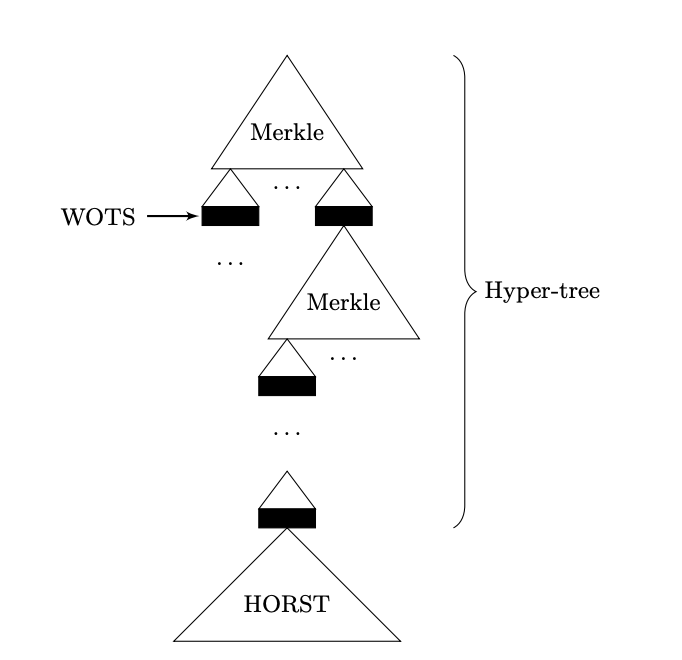
\includegraphics[scale=1]{SPHINCS.png}
    \caption{Пример SPHINCS. Гипердерево состоит из $d$ слоев дерева Меркля и соединены WOTS. Внизу дерево HORS(или HORST) соединяется с подписанным сообщением.}
    \label{fig:SPHINCS}
\end{figure}

\begin{enumerate}
    \item Главное Гипердерево, высотой $h$ (60 в SPHINCS-256). Корень этого дерева является частью открытого ключа. Листья этого дерева экземпляры HORST. Это Гипердерево делится на $d$ слоев($d$ = 12 в SPHINCS-256).
    \item Поддеревья, которые являются деревьями Меркля высоты $h/d$ (60/12 = 5 в SPHINCS-256). Листья этих деревьев являются корнями деревьев; указанные корни являются сжатыми открытыми ключами экземпляров WOTS, которые соединяются с деревом на следующем уровне.
    \item Открытый ключ WOTS это деревья сжатия, которые являются \newline L-деревьями, высоты $\lceil log_{2}l \rceil$.Листья этого дерева являются компонентами WOTS открытого ключа (67 значений по 256 бит каждое в SPHINCS-256). Связанный экземпляр WOTS подписывает корень дерева на следующем уровне.
    \item В нижней части гипердерева, открытый ключ HORST --- деревья сжатия это деревья Меркля высоты $\tau = log_{2}t$, где $t$ номер элементов открытого ключа HORST($2^{16}$ в SPHINCS-256).
\end{enumerate}

Алгоритм Sign в SPHINCS формально можно описать:

\begin{enumerate}
    \item Извлекается листовой индекс из сообщения и личного ключа. Этот индекс определяет один из экземпляров $2^{h}$ HORST (относительно основного гипердерева), который будет использоваться для подписи сообщения.
    \item Создайте экземпляр HORST, который является производным от личного ключа и конечного индекса, и подпишите сообщение этим экземпляром HORST. Подпись HORST включает $k$ ключей и их соответствующие пути аутентификации и является частью подписи SPHINCS. Итого получаем сжатый в дереве HORST открытый ключ $p$.
    \item Для каждого слоя гипердерева подпишите открытый ключ $p$(полученный из нижнего слоя), используя правильный экземпляр WOTS(полученный из листового индекса); добавьте эту подпись WOTS и связанный с ней путь аутентификации к подписи SPHINCS. Вычислите путь аутентификации этого экземпляра WOTS в поддереве. Добавьте этот путь к подписи SPHINCS и $p$-корень поддерева.
\end{enumerate}

\subsection{Gravity-SPHINCS}
\label{gravity-sphincs}
Gravity-SPHINCS \cite{stateless}, схема подписи на основе SPHINCS с более короткими ключами (32 и 64 байта вместо $\approx$ 1 КБ), более короткими подписями ($\approx$ 30 КБ вместо 41 КБ) и более быстрыми алгоритмами Sign и Verify.
Gravity-SPHINCS наследует некоторые параметры от SPHINCS (длина хэша, глубина WOTS и др.), а так же имеет новые. В приведенном ниже списке $h$ обозначает высоту поддеревьев(в отличие от высоты основного дерева в SPHINCS), а $B_{n} = \{0,1\}^{n}$ обозначает набор $n$-битовых блоков.
\newline

Параметры являются следующими:

\begin{itemize}
    \item Хэш-выход длина бита $n$, положительное целое число.
    \item Глубина WOTS $w$, степень 2-ки такой, что $w \geq 2$ и $log_{2}w$ делит $n$.
    \item Размер множества PORS $t$, положительное, степень двойки.
    \item Размер подмножества PORS $k$, положительное целое такое, что $k \leq t$.
    \item Высота дерева Меркля $h$, положительное целое.
    \item Количество внутренних деревьев Меркля $d$, неотрицательное целое.
    \item Высота кэша $c$, неотрицательное целое.
    \item Высота $b$, неотрицательное целое.
    \item Пространство сообщения $M$, обычно подмножество битовых блоков $\{0,1\}^{*}$.
\end{itemize}

Из этих параметров получены:

\begin{itemize}
    \item Размер WOTS $l = \mu + \lfloor log_{2}(\mu(w - 1))/log_{2}w \rfloor + 1$, где $\mu = n/log_{2}w$.
    \item Множество PORS, $T = \{0, ..., t - 1\}$.
    \item Адресное пространство $A = \{0, ..., d\} \times \{0, ..., 2^{c + dh} - 1\} \times \{0, ..., max(l,t) - 1\}$.
    \item Пространство открытых ключей $PK = B_{n}$.
    \item Пространство личных ключей $SK = B^{2}_{n}$.
    \item Пространство подписи $SG = B_{n} \times B^{k}_{n} \times B^{\leq k(log_{2}t - \lfloor log_{2}k \rfloor)}_{n} \times (B^{l}_{n} \times B^{h}_{n})^{d} \times B^{c}_{n}$.
    \item $SG_{B} = B^{b}_{n} \times \{0, ..., 2^{b} - 1\} \times SG$
    \item Размер открытого ключа $n$ бит.
    \item Размер личного ключа, $2n$ бит.
    \item Максимальный размер подписи
    \[sigsz = (1 + k +k(log_{2}t - \lfloor log_{2}k \rfloor) + d(l + h) + c)n\]
\end{itemize}

Алгоритм подписи $Sign$ одного сообщения и проверка $Verify$ в Gravity-SPHINCS очень похожа на SPHINCS.
\newline

Опишем три алгоритма подписи Gravity-SPHINCS:

\begin{itemize}
    \item Алгоритм генерации ключей Gen:

    \begin{itemize}
        \item Вход: $2n$ случайных бит, где $n$ --- параметр безопасности.
        \item Выход: Личный ключ $sk \in B^{2}_{n}$, и открытый ключ $pk \in B_{n}$.
        \item Шаги:

        \begin{enumerate}
            \item Генерация личного ключа из $2n$ случайных бит:
            \[sk = (seed, salt) \stackrel{\$}{\leftarrow} B^{2}_{n}\]
    
            \item Для $0 \leq i < 2^{c+h}$ генерируется WOTS открытый ключ:
            \[x_{i} \leftarrow WOTS, \text{используя } genpk(seed, make-addr(0, i))\]
    
            \item Генерация открытого ключа:
            \[pk \leftarrow Merkle, \text{используя } root_{c+h}(x_{0}, ..., x_{2^{c+h} - 1})\]
        \end{enumerate}
    \end{itemize}

    \item Алгоритм подписи Sign:

    \begin{itemize}
        \item Вход: Хэш $m \in B_{n}$ и личный ключ $sk = (seed, salt)$
        \item Выход: Подпись $\sigma$.
        \item Шаги:

        \begin{enumerate}
            \item Вычисляем $s \leftarrow H(salt, m)$.
    
            \item Вычисляем гипердерева индекс и случайное подмножество как
            \[j, (x_{1}, ..., x_{k}) \leftarrow PORS(s, m)\]
    
            \item Вычисляем PORST подпись и открытый ключ:
            \[(\sigma_{d}, oct, p), \text{используя } sign(seed, make-addr(d, j), x_{1}, ..., x_{k})\]
    
            \item Для $i \in \{d - 1, ..., 0\}$ выполняется:
            
            \begin{enumerate}
                \item Вычисляем WOTS подпись:
                \[\sigma_{i} \leftarrow WOTS, \text{используя } sign(seed, make-addr(i,j),p)\]
    
                \item Вычисляем $p \leftarrow WOTS, \text{используя } extractpk(p, \sigma_{i})$.
    
                \item $j^{*} \leftarrow \lfloor j / 2^{h} \rfloor$.
    
                \item Для $u \in \{0, ..., 2^{h} - 1\}$ вычислим WOTS открытый ключ:
                \[p_{u} \leftarrow WOTS, \text{используя } genpk(seed, make-addr(i, 2^{h}, j^{*} + u))\]
    
                \item Вычислим Меркля путь аутентификации:
                \[A_{i} \leftarrow Merkle, \text{используя } auth_{h}(p_{0}, ..., p_{2^{h} - 1}, j - 2^{h}j^{*})\]
    
                \item $j \leftarrow j^{*}$.
            \end{enumerate}
    
            \item Для $0 \leq u < 2^{c+h}$ вычислим WOTS открытый ключ:
            \[p_{u} \leftarrow WOTS, \text{используя } genpk(seed, make-addr(0, u))\]
    
            \item Вычислим Меркля путь аутентификации:
            \[(a_{1}, ..., a_{h+c}) \leftarrow Merkle, \text{используя } auth_{h+c}(p_{0}, ..., p_{2^{h+c} - 1}, 2^{h}j)\]
    
            \item $A_{c} \leftarrow (a_{h+1}, ..., a_{h+c})$.
    
            \item Получаем подпись $(s, \sigma_{d}, oct, \sigma_{d - 1}, A_{d - 1}, ..., \sigma_{0}, A_{0}, A_{c})$.
        \end{enumerate}
    \end{itemize}

    \item Алгоритм проверки подписи Verify:

    \begin{itemize}
        \item Вход: Хэш $m \in B_{n}$, открытый ключ $pk \in B_{n}$ и подпись
        \[(s, \sigma_{d}, oct, \sigma_{d - 1}, A_{d - 1}, ..., \sigma_{0}, A_{0}, A_{c})\]
        \item Выход: 1 (подпись корректна) или 0 (нет).
        \item Шаги:

        \begin{enumerate}
            \item Вычислим индекс гипердерева и случайное подмножество
            \[j, (x_{1}, ..., x_{k}) \leftarrow PORS(s,m)\]
    
            \item Вычислим открытый ключ PORST,
            \[p \leftarrow PORST, \text{используя } extractpk(x_{1}, ..., x_{k}, \sigma_{d}, oct).\]
    
            \item Если $p = \perp$, затем прерываем и возвращаем 0.
    
            \item Для $i \in \{d - 1, ..., 0\}$ выполняем следующее:
    
            \begin{enumerate}
                \item Вычислим открытый ключ WOTS:
                \[p \leftarrow WOTS, \text{используя } extractpk(p, \sigma_{i})\]
                \item $j^{*} \leftarrow \lfloor j/2^{h} \rfloor$.
                \item Вычислим корень дерева Меркля:
                \[p \leftarrow Merkle, \text{используя } extract_{h}(p, j - 2^{h}j^{*}, A_{i})\]
                \item $j \leftarrow j^{*}$.
            \end{enumerate}
    
            \item Вычислим корень дерева Меркля:
            \[p \leftarrow Merkle, \text{используя } extract_{c}(p, j, A_{c})\]
    
            \item В результате 1, если $p = pk$ и 0 в ином случае.
        \end{enumerate}
    \end{itemize}

    
\end{itemize}

\subsection{$\text{SPHINCS}^{+}$}
\label{sec_sphincsplus}
Хотя в практическом плане размер подписи и скорость SPHINCS далеки от того, к чему мы привыкли, от подписей RSA или ECDSA. В данной работе представлен алгоритм $\text{SPHINCS}^{+}$ \cite{stateless}, который улучшает SPHINCS с точки зрения скорости алгоритмов схемы и размера подписи.

$\text{SPHINCS}^{+}$ использует псевдослучайную функцию $PRF$ для генерации ключей, $PRF : \{0, 1\}^{n} \times \{0, 1\}^{256} \rightarrow \{0, 1\}^{n}$, и псевдослучайную функцию $PRF_{msg}$ для генерации случайного сжатия сообщения: $PRF_{msg} : \{0, 1\}^{n} \times \{0, 1\}^{n} \times \{0, 1\}^{*} \rightarrow \{0, 1\}^{n}$. Для сжатия подписываемого сообщения мы используем дополнительную хэш-функцию $H_{msg}$, которая может обрабатывать сообщения произвольной длины:
\[H_{msg} : \{0, 1\}^{n} \times \{0, 1\}^{n} \times \{0, 1\}^{n} \times \{0, 1\}^{*} \rightarrow \{0, 1\}^{m}\]

$\text{SPHINCS}^{+}$ Личный и открытый ключ:

\begin{itemize}
    \item Открытый ключ состоит из двух $n$-битных значений: корневого узла из трех верхних в гипердереве и случайного открытого начального значения $PK$.
    \item Личный ключ состоит еще из двух $n$-битных случайных: $SK$, чтобы генерировать $\text{WOTS}^{+}$ и $FORS$ личные ключи, и $SK.prf$, используемый ниже для случайного хэша сообщения.
\end{itemize}

$\text{SPHINCS}^{+}$ Подпись сообщения.

Как не удивительно, что подпись состоит из FORS подписи для хэша сообщения, $\text{WOTS}^{+}$ подпись соответствующих открытых ключей FORS, ряда каналов аутентификации для подтверждения того, что $\text{WOTS}^{+}$ является открытым ключом. Чтобы проверить эту цепочку путей и подписей, проверка итеративно восстанавливает открытые ключи и корневые узлы до тех пор, пока не будет достигнут корневой узел в верхней части гипердерева $\text{SPHINCS}^{+}$. 
\newline

Расмотрим два момента из алгоритма:

\begin{itemize}
    \item Вычисление хэша сообщения.
    \item Выбор листа.
\end{itemize}

Здесь $\text{SPHINCS}^{+}$ отличается от оригинальных SPHINCS тонкими, но важными деталями.

Во-первых, мы псевдо случайным образом генерируем случайные числа $R$, основанные на сообщении и $SK.prf$. $R$ может быть дополнительно сконструирован недетерминированным путем добавления дополнительной случайности $OptRand$. Это может противодействовать атакам бокового канала, которые полагаются на сбор нескольких следов для одного и того же вычисления. Обратите внимание, что установка этого значения в нулевую строку (или использование значения с низкой энтропией) не оказывает отрицательного влияния на псевдослучайность $R$. Формально, мы полагем, что $R = PRF(SK.prf, OptRand, M)$. $R$ часть подписи. Используя $R$, мы затем получаем индекс конечного узла, который должен использоваться, а также получаем хэш-значение сообщения $(MD||idx) = H_{msg}(R, PK, PK.root, M)$.

В отличие от SPHINCS, этот метод выбора индекса является публично проверяемым, не позволяя злоумышленнику свободно выбирать кажущийся случайным индекс и комбинировать его с сообщением по своему выбору. Критически важно, что это противодействует многоцелевым атакам на схему подписи $FTS$. Поскольку индекс теперь может быть вычислен верификатором, он больше не включается в подпись.
\newpage

% Введение в Bitshares
\section{Программная реализация}
В распределенной базе данных блокчейн используются подпись на эллиптических кривых ECDSA (Elliptic Curve Digital Signature Algorithm) с кривой $secp256k1$ для подписания транзакций и отправки их в сеть. Реализованы подписи на основе функций хэширования без состояния, (SPHINCS, $\text{SPHINCS}^{+}$, Gravity-SPHINCS) на языке Python. А также данные системы ЭЦП интегрированы в современную блокчейн-систему под названием Bitshares, заменив подпись на эллиптических кривых.

\subsection{Введение в блокчейн Bitshares}
В 2013 году под авторством Даниила Ларимера была опубликована статья с упоминанием Bitshares. Идея протокола Bitshares состоит в создании платформы, с помощью которой можно было бы торговать разными активами и валютами в децентрализованной среде.

\subsection{Назначение платформы Bitshares}
Протокол реализует децентрализованную биржу, где этими цифровыми активами можно торговать. При проектировании учетной системы и механизма достижения консенсуса разработчики сделали большой упор на пропускную способность. Как результат, Bitshares позиционирует себя как децентрализованная альтернатива учетной системе $Visa$. В то время как $Visa$ заявляет, что может обрабатывать пару десятков тысяч транзакций в секунду, Bitshares говорит о способности обрабатывать сто тысяч транзакций в секунду, причем децентрализованным образом, с открытой базой данных и возможностью аудита.

\subsection{Достижение консенсуса на основе DPoS}
Правила работы протокола DPoS (Delegated Proof of Stake) предполагают, что все пользователи могут принимать участие в достижении консенсуса, выбирая валидаторов посредством голосования. В процессе голосования вес голоса пользователя определяется его балансом в базовой валюте. Формирование блоков выполняется подмножеством избранных валидаторов. В рамках протокола Bitshares валидатор называется $witness$.

\subsection{Модель транзакций}
Детальнее остановимся на модели транзакций в Bitshares. Так как основная работа заключалась в замене подписи транзакций в данной платформе на подписи на основе функций хэширования без состояния. (см. Рис. \ref{fig:Bitshares_trx_model}).

\begin{figure}[h]
    \centering
    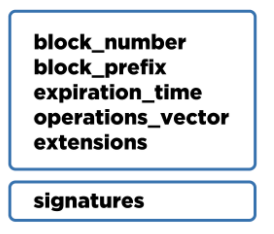
\includegraphics[scale=0.5]{Bitshares_trx_model.png}
    \caption{Модель транзакции в Bitshares}
    \label{fig:Bitshares_trx_model}
\end{figure}

На схеме видно, что тело транзакции состоит из пяти основных полей. Первые два поля транзакции необходимы для того, чтобы привязать ее к определенному блоку. Это нужно, чтобы определить цепочку блоков, в которую эта транзакция может быть добавлена, поскольку по правилам протокола транзакция не может быть подтверждена в той цепочке, к которой не привязана. Поле $expiration\_time$ задает время, до которого транзакция может быть добавлена в блок. Если она не была подтверждена до наступления этого времени, то она считается невалидной и уже не может быть включена в блокчейн.

Поле $operations\_vector$ является особенным. Эта особенность состоит в том, что в него можно поместить много разных операций. Операция — это еще один ключевой объект в протоколе Bitshares. Назовем несколько самых популярных типов операций: $transfer$ (перевод), $account\_update$ (обновление аккаунта), $asset\_issue$ (выпуск токена) Каждая операция имеет свой формат и необходимые параметры. Например, операция $transfer$ требует указания аккаунта отправителя, типа актива, суммы перевода и аккаунта получателя. Сами операции независимы друг от друга, но могут быть выполнены только вместе, если транзакция будет принята. То есть мы можем сделать несколько переводов средств между аккаунтами и выпустить все эти переводы одной транзакцией.

Поле $extensions$ сделано для обратной совместимости, чтобы текущая версия программного обеспечения могла обрабатывать транзакции новой версии, где могут быть добавлены дополнительные поля. Конечно же, старое ПО не будет знать, как правильно верифицировать дополнительные поля новых транзакций, но хотя бы сможет корректно обрабатывать транзакции согласно старым правилам.

Это формат неподписанной транзакции. Для того чтобы транзакцию правильно подписать, нужно проанализировать все операции из $operations\_vector$ и составить список аккаунтов, которые должны подтвердить данную транзакцию. Тогда станет ясно, какими ключами нужно подписывать транзакцию. Все необходимые подписи помещаются в отдельное поле — $signatures$. Если не будет хватать хотя бы одной подписи, то вся транзакция будет считаться неправильной.

Отметим, что за счет оптимизации размера идентификаторов финальный размер транзакции, которая содержит одну операцию будет равен приблизительно 100 байт. Это действительно очень компактная транзакция, если сравнить ее с транзакцией в других протоколах.

Что касается комиссионных сборов, то в протоколе Bitshares реализован особый подход, называется он $fee$. Каждая операция требует определенной оплаты, которая снимается с баланса аккаунта инициатора в момент подтверждения транзакции. Комиссия за осуществление операций может быть постоянной, а может меняться. В качество грубого сравнения можно отметить, что комиссии за обычные переводы и торговлю значительно ниже, чем комиссии за выпуск новых активов и регистрацию нового аккаунта.

\subsection{Взаимодействие с Bitshares}
$API$ Bitshares доступны с помощью удаленных вызовов процедур($RPC$) и вызовов и уведомлений $WebSocket$. Все вызовы $API$ форматируются в формате $JSON$ и возвращают только $JSON$. Ссылки на $API$ Bitshares-$Core$ находятся в документации $Doxygen$, которая генерируется для каждой версии Bitshares на языке $Perl$. Кроме того, вы можете найти информацию о классах, компонентах и элементах $API$ в подробной и структурной документации Bitshares.

$API$ --- интерфейсы разделяются на две категории, а именно:

\begin{itemize}
    \item $Blockchain$ $API$ --- используется для запроса блокчейн-данных(счета, активы, торговая история и так далее). Кроме того, данные хранятся в самом блокчейне (блоки, транзакции и так далее), объекты более высокого  (например, счета, балансы и так далее) можно получить через полную базу данных узла.
    \item $Wallet$ $API$ – отдельный модуль взаимодействия с блокчейном, для удобство разработчиков и тестирование новых операций.
\end{itemize}

Кошелек ($cli$-$wallet$) имеет ваши личные ключи и возможности подписи. Он требует работающего полного узла ($witness$) (не обязательно локально) и подключается к нему. Потому что кошелек не предлагает возможности $P2P$ или $blockchain$ напрямую.

\subsection{Одноранговый сетевой протокол Bitshares}
Узлы Bitshares взаимодействуют друг с другом через одноранговый сетевой протокол ($P2P$).

Каждый узел принимает соединения через $TCP$-сокет(не обязательно открытый). Сразу же после установления соединения узлы обмениваются криптографическими ключами, которые впоследствии используются для шифрования трафика внутри этого соединения.

Протокол состоит из сообщений, которыми обмениваются через зашифрованное соединение. Протокол поддерживает различные типы сообщений для запроса информации или передачи элементов блокчейна.

\subsubsection{Коммуникационные уровни}

\begin{itemize}
    \item Уровень шифрования

    Весь сетевой трафик после первоначального обмена ключами шифруется с помощью $AES-256$.

    Для обмена ключами каждый узел создает случайный личный ключ на кривой $secp256k1$, вычисляет соответствующий открытый ключ и передает его в открытом виде по соединению.

    После получения удаленного открытого ключа он умножается на собственный личный ключ. Результирующая точка кривой хэшируется с помощью $SHA-512$, чтобы получить общий хэш 512 бит.

    Из этого общего секрета создается 256-битный ключ путем хэширования его с помощью $SHA-256$. Аналогично, 128-битный создается путем хэширования секрета с помощью $city\_hash\_128$. 256-битный ключ и 128-битный затем используются для настройки потоков шифрования и расшифрования $AES-256-CBC$ для отправки и приема данных.
    \item Уровень обмена сообщениями

    Сообщения состоят из заголовка 8 байт (4 байта $little$-$endian$ целочисленного размера, 4 байта $little$-$endian$ целочисленного типа) плюс фактическое содержимое сообщения. Содержимое представляет собой двоичное сериализованное представление структуры данных, обозначенной полем тип.

    Для передачи сообщения дополняются кратным 16 байтам. (16 байт --- это размер блока, обрабатываемого базовыми потоками $AES$. Таким образом, сообщения всегда могут быть зашифрованные или расшифрованными без необходимости ждать дальнейших данных.)
\end{itemize}

\subsubsection{Жизненный цикл подключения}
$P2P$ --- соединения, как правило, долговечны. Узел будет пытаться подключиться к определенному минимальному числу одноранговых узлов и может принимать дополнительные соединения до определенного максимального числа. Узлы разъединяются только тогда, когда они в каком-то смысле плохо себя ведут, то есть вредят сети отправляя некорректные данные.

% Интеграция языков программирования
\subsection{Интеграция языков программирования}
В данной работе, реализация подписей на основе функций хэширования использовался $Python$, в том время, когда платформа Bitshares написана на $C++$. Поэтому появилась необходимость интегрировать $Python$ в проект Bitshares.
Для интеграции $C++$ кода в $Python$ используется библиотека $Boost.Python$. Однако в данной работе потребовалось сделать обратное: вызвать код $Python$ со стороны $C++$. Это требует встроить интерпретатор $Python$ в $C++$ программу.

В настоящее время $Boost.Python$ не поддерживает напрямую все, что нужно при встраивании. Поэтому нужно использовать $API Python / C$ для заполнения пробелов. Тем не менее, $Boost.Python$ уже значительно упрощает встраивание и в будущей версии может вообще не потребоваться касаться $API Python / C$.

\subsubsection{Сборка встроенных программ}
Чтобы иметь возможность встраивать $Python$ в свои программы, мы должны ссылаться как на $Boost.Python$, так и на собственную библиотеку времени выполнения $Python$.

Библиотека $Boost.Python$ поставляется в двух вариантах. Оба находятся в $/libs/python/build/bin.stage$ подкаталоге $Boost$. В $Windows$ варианты называются $boost\_python.lib$(для выпусков сборки) и $boost\_python\_debug.lib$(для отладки). Если вы не можете найти библиотеки, возможно, вы еще не создали $Boost.Python$.

Библиотека $Python$ находится в $/libs$ подкаталоге вашего каталога $Python$. В $Windows$ это называется $pythonXY.lib$, где $XY$ --- ваш основной номер версии $Python$.

Кроме того, $/include$ подкаталог $Python$ должен быть добавлен в ваш путь включения.

В $Jamfile$(краткое описание вышеперечисленного) сводится к:
\begin{verbatim}
    Projectroot c:\projects\embedded_program ;

    SEARCH on python.jam = $(BOOST_BUILD_PATH) ;
    include python.jam ;

    exe embedded_program
    : #sources
        embedded_program.cpp
    : # requirements
        <find-library>boost_python <library-path>c:\boost\libs\python
    $(PYTHON_PROPERTIES)
        <library-path>$(PYTHON_LIB_PATH)
        <find-library>$(PYTHON_EMBEDDED_LIBRARY) ;
\end{verbatim}

\subsubsection{Подготовка к работе}
Для встраивания интерпретатора $Python$ в одну из программ на $C++$ необходимо выполнить следующие 3 шага:

1. Подключить $\#include <boost/python.hpp>$.

2. Вызовите $Py\_Initialize()$ для запуска интерпретатора и создать $\_\_main\_\_$  модуль.

3. Вызовите другие процедуры $API\ Python\ C$, чтобы использовать интерпретатор.

\subsubsection{Использование интерпетатора}
Объекты в $Python$ подсчитываются по ссылкам. Естественно, $PyObjectAPI$ $Python$ $C$ также подсчитываются по ссылкам. Однако есть разница. Хотя подсчет ссылок в Python полностью автоматический, $API$-интерфейс $Python$ $C$ требует, чтобы вы делали это вручную . Это грязно и особенно трудно понять в присутствии исключений $C++$. К счастью, $Boost.Python$ предоставляет шаблоны дескрипторов и классов объектов для автоматизации процесса.

\subsubsection{Запуск кода Python}
$Boost.python$ предоставляет три связанные функции для запуска кода $Python$ из $C++$.
\verbatimfont{\small}
\begin{verbatim}
    object eval(str expression, object globals = object(), object locals = object())
    object exec(str code, object globals = object(), object locals = object())
    object exec_file(str filename, object globals = object(), object locals = object())
\end{verbatim}

\begin{enumerate}
    \item $eval$ вычисляет выражение и возвращает полученное значение.
    \item $exec$ выполняет данный код(обычно набор операторов), возвращающий результат.
    \item $exec\_file$ выполняет код, содержащийся в данном файле.
\end{enumerate}

Параметры $globals$ и $locals$ --- это словари $Python$, содержащие глобальные и локальные значения контекста, в котором выполняется код. Вы можете использовать пространство имен модуля $\_\_main\_\_$ для обоих параметров.

$Boost.python$ предоставляет функцию для импорта модуля:
\begin{verbatim}
    object import(str name)
\end{verbatim}

$import$ импортирует модуль $python$(потенциально загружая его сначала в запущенный процесс) и возвращает его.

Давайте импортируем модуль $\_\_main\_\_$ и запустим некоторый код $Python$ в его пространстве имен:

\begin{verbatim}
    object main_module = import("__main__");
    object main_namespace = main_module.attr("__dict__");

    object ignored = exec("hello = file('hello.txt', 'w')\n"
                        "hello.write('Hello world!')\n"
                        "hello.close()",
                        main_namespace);
\end{verbatim}

В итоге получаем файл под названием $"hello.txt"$ в текущем каталоге, содержащем фразу, которая хорошо известна в кругах программирования.

% Результаты
\subsection{Результаты}
Создание на Macbook Pro(3.1 GHz i5, 8GB оперативной памяти), пар ключей одноразовой подписи и дерева сертификации Меркля разных размеров дало следующие результаты(WOTS): $2^4 = 0.465s, 2^5 = 1.135s, 2^6 = 3.650s, 2^8 = 14.540s$. Создание гипердерева, состоящего из начальной генерации двух $2^4$ деревьев, занимает около 1 секунды по сравнению с $~14s$, требующимися для генерации стандартного $2^8$ дерева $MSS$ для одного и того же объема подписей. 

Общая идея гипердерева состоит в том, что корень дочернего дерева Меркля подписывается ключом одноразовой подписи из хэша листа родительского дерева Меркля, известного как дерево сертификации. Проблема с базовой $MSS$ заключается в том, что количество доступных подписей ограничено, и все пары ключей одноразовых подписей должны быть предварительно сгенерированы до вычисления дерева Меркля. Генерация ключей и время подписания растут экспоненциально относительно высоты дерева, $h$, что означает, что деревья, превышающие 256 ключей одноразовой подписи, становятся затратными по параметрам времени и вычислительной мощности, необходимых для генерации. Стратегия отсрочки вычислений при генерации ключей и деревьев, а также расширение количества доступных пар ключей одноразовой подписи заключается в использовании дерева, которое само состоит из деревьев Меркля, называемого гипердеревом. Размер подписей растет линейно для каждого дополнительного дерева, которое подписывается, в то время как объём подписей гипердерева увеличиваентся экспоненциально.

Увеличение глубины(или высоты) гипердерева продолжает эту тенденцию. Гипердерево, состоящее из четырех соединенных $2^4$ деревьев сертификации и дерева подписи размером $2^4$, может содержать $2^{20} = 1 048 576$ подписей с увеличенным размером подписи, но при этом время создания составляет всего $2.420s$.

Нет необходимости, чтобы гипердерево было симметричным, и поэтому, если оно состояло первоначально из двух деревьев, оно может быть расширено впоследствии путем присоединения дополнительных слоев деревьев. Таким образом, подписи блока транзакций будут изначально небольшого размера, который будет постепенно возрастать по мере увеличения глубины гипердерева. Использование гипердерева Меркля для создания и подписи адреса блока транзакций вряд ли потребуется для количества транзакций превышающего $2^{12}$. Таким образом, возможность создать с вычислительной легкостью $2^{20}$ защищенных подписей для глубины гипердерева $h = 5$ является более чем достаточной.

Использование схемы подписи Меркля $MSS$ безопасно основывается на неиспользовании повторно ключей одноразовой подписи. Таким образом, это зависит только от состояния подписей или записей о подписанных транзакциях. Как правило, в реальном мире это потенциально может быть проблемой, но неизменяемый открытый блок цепочки транзакций является идеальным хранилищем для криптографической схемы подписи с учетом состояния. В 2015 году стало известно о новой схеме криптографической подписи на основе функций хэширования под названием SPHINCS (с алгоритмом подписи можно ознакомится выше), которая предлагает практически не зависящие от состояния подписи с $2^{128}$-битной защитой.

Чтобы получить контрольные показатели, мы оцениваем реализацию на компьютере используя набор инструкций Intel x86-64. В частности, используем одноядерный процессор $Intel$ $Core$ $i5$ с частотой 3,1 ГГц. Мы следуем стандартной практике отключения $TurboBoost$ и $hyper-threading$, для чистоты эксперимента. Система имеет 32 КБ кэша инструкций $L1$, 32 КБ кэша данных $L1$, 256 КБ кэша $L2$ и 8192 КБ кэша $L3$. Кроме того, система имеет 8 ГБ оперативной памяти. При выполнении тестов производительности система работала на ядре $Linux 4.9.0-4-amd64$. Для компилиляции кода, использовался $GCC$ версии 8.3.0, с флагом оптимизации компилятора.
\newline

\begin{table}[h!]
    \begin{center}
      \caption{Сравнение быстродействия}
      \label{tab:table1}
      \begin{tabular}{l|c|c|c}
        \textbf{Система} & \textbf{Gen} & \textbf{Sign} & \textbf{Verify}\\
        \hline
        SPHINCS-256 & 12.6 ms & 236 ms & 2.73 ms\\
        $\text{SPHINCS}^+$ & 11.7 ms & 196 ms & 2.3 ms\\
        Gravity-SPHINCS & 10.3 ms & 204 ms & 2.4ms\\
        ECDSA(P-256) & 0.924 ms & 0.553 ms & 0.478 ms\\
      \end{tabular}
    \end{center}
  \end{table}
\newpage

% Заключение
\section{Заключение}
В дипломной работе получены следующие результаты:
\begin{enumerate}
    \item Подготовлен обзор публикаций по основам HBC (Hash-Based\\ Cryptography).
    \item Изучены современные алгоритмы электронных цифровых подписей на основе функций хэширования.
    \item Реализованы программные реализации (язык Python) WOTS, $\text{WOTS}^+$, HORS, SPHINCS, $\text{SPHINCS}^+$, Gravity-SPHINCS.
    \item Реализации SPHINCS, $\text{SPHINCS}^+$, Gravity-SPHINCS успешно интегрированы в блокчейн архитектуру Bitshares.
    \item Проведена оценка быстродействия разработанных реализаций в сравнении с подписью на эллиптических кривых ECDSA для подписи транзакции (См. таблицу \ref{tab:table1}).
\end{enumerate}

Исходя из нашей работы, подписи на основе функций хэширования не идеальны, так как требуют большего времени на генерацию ключей, подпись и проверку, чем нынешние решения на эллиптических кривых. А также существует проблема и с хранением самих подписей, они требуют больше затрат по памяти, но несмотря на это они обеспечивают безопасность данных, что важнее в наше время. У нас получилось реализовать электронные цифровые подписи на основе функций хэширования без состояния, такие как SPHINCS-256, $\text{SPHINCS}^+$, Gravity-SPHINCS для подписания транзакций и интегрировать в существующий протокол блокчейна под названием Bitshares и провести оценку быстродействия разработанных реализаций.
\newpage

% Cписок литературы
\begin{thebibliography}{9}
    \bibitem{latexcompanion}
    Security of One-Time Signatures under Two-Message Attacks. Andreas Hülsing,
    \texttt{https://eprint.iacr.org/2016/1042.pdf}.
    
    \bibitem{wots}
    On the Security of the Winternitz One-Time Signature Scheme. Johannes Buchmann, Erik Dahmen, Sarah Ereth,
    \texttt{https://eprint.iacr.org/2010/446.pdf}.

    \bibitem{knuthwebsite}
    Short One-Time Signatures. Gregory M. Zaverucha and Douglas R. Stinson.
    \texttt{https://eprint.iacr.org/2011/191.pdf}.

    \bibitem{wotsplus}
    $\text{WOTS}^{+}$ – Shorter Signatures for Hash-Based Signature Schemes. Andreas Hulsing,
    \texttt{https://eprint.iacr.org/2017/965.pdf}.

    \bibitem{stateless}
    Proof-of-forgery for hash-based signatures. E.O. Kiktenko, M.A. Kudinov, A.A. Bulychev, and A.K. Fedorov,
    \texttt{https://arxiv.org/pdf/1905.12993.pdf}.

    \bibitem{imrstateless}
    Improving Stateless Hash-Based Signatures. Jean-Philippe Aumasson and Guillaume Endignoux,
    \texttt{https://eprint.iacr.org/2017/933.pdf}.

    \bibitem{sphincsplus}
    The $\text{SPHINCS}^{+}$ Signature Framework. Daniel J. Bernstein,
    \texttt{https://eprint.iacr.org/2019/1086.pdf}.
\end{thebibliography}
\addcontentsline{toc}{section}{\protect\numberline{}Список литературы}
\newpage

% Приложение
\section*{Приложение}
\addcontentsline{toc}{section}{\protect\numberline{}Приложение}
\textbf{Пример реализации SPHINCS-256 на языке Python}
\begin{verbatim}

import hmac
import hashlib
from binascii import unhexlify, hexlify
from math import ceil, floor, log
import time
from os import urandom
import sys

class WOTS(object):

    def random_key(n=32):  # returns a 256 bit hex encoded (64 bytes) random number
        return hexlify(urandom(n))
    
    
    def sha256(message):
        return hashlib.sha256(message).hexdigest()
    
    
    def sha256b(message):
        return hashlib.sha256(message).digest()
    
    
    def random_wkey(w=8, verbose=0):  # create random W-OTS keypair
        priv = []
        pub = []
        print("Hashing number random keys by:\t", 2**w)
        for _ in range(256/w):
            a = random_key()
            priv.append(a)
            for _ in range(2**w-1):
                a = sha256(a)
            pub.append(sha256(a))
    
        return priv, pub
    
    
    def sign_wkey(priv, message):
        signature = []
        bin_msg = unhexlify(sha256(message))
    
        for y in range(len(priv)):
            s = priv[y]
            for _ in range(256-ord(bin_msg[y:y+1])):
                s = sha256(s)
            signature.append(s)
        return signature
    
    
    def verify_wkey(signature, message, pub):
        verify = []
        bin_msg = unhexlify(sha256(message))
    
        for x in range(len(signature)):
            a = signature[x]
            for _ in range(ord(bin_msg[x:x+1])):
                a = sha256(a)
            verify.append(a)
    
        if pub != verify:
            return False
    
        return True

class HORS(object):
    def get_private():
    priv = []
    for x in range(nvals):
        priv.append(random.randint(0, max))
    return priv


    def int_to_bytes(value):
        result = bytearray()

        for i in range(0, len(value)/2):
        str = value[2*i:2*i+2]
            result.append(int(str, 16))
        result.reverse()

        return result


    def hashthem(priv):
        pub = []

        for x in priv:
        m = hashlib.md5()
        m.update(str(x))
        pub.append(m.hexdigest()[:4])
        return pub


    def getsig(val, priv, pub):
        sig = []
        for x in val:
        sig.append(pub[priv[x]])
        return sig

from ChaCha import ChaCha
from HORS import HORS
from bytes_utils import xor
from blake import BLAKE
from trees import l_tree, hash_tree, auth_path, construct_root, root

class SPHINCS(object):

    #    def __init__(self, n=256, m=512, h=60, d=12, w=16, tau=16, k=32):
    def __init__(self, n=256, m=512, h=60, d=12, w=16, tau=16, k=32):

        self.n = n
        self.m = m
        self.h = h
        self.d = d
        self.w = w
        self.tau = tau
        self.t = 1 << tau
        self.k = k

        self.Hdigest = lambda r, m: BLAKE(512).digest(r + m)
        self.Fa = lambda a, k: BLAKE(256).digest(k + a)
        self.Frand = lambda m, k: BLAKE(512).digest(k + m)

        C = bytes("expand 32-byte to 64-byte state!", 'latin-1')
        perm = ChaCha().permuted
        self.Glambda = lambda seed, n: ChaCha(key=seed).keystream(n)
        self.F = lambda m: perm(m + C)[:32]
        self.H = lambda m1, m2: perm(xor(perm(m1 + C), m2 + bytes(32)))[:32]

        self.wots = WOTSplus(n=n, w=w, F=self.F, Gl=self.Glambda)
        self.horst = HORST(n=n, m=m, k=k, tau=tau,
                           F=self.F, H=self.H, Gt=self.Glambda)

    def address(self, level, subtree, leaf):
        t = level | (subtree << 4) | (leaf << 59)
        return int.to_bytes(t, length=8, byteorder='little')

    def wots_leaf(self, address, SK1, masks):
        seed = self.Fa(address, SK1)
        pk_A = self.wots.keygen(seed, masks)

        def H(x, y, i): return self.H(xor(x, masks[2*i]), xor(y, masks[2*i+1]))
        return root(l_tree(H, pk_A))

    def wots_path(self, a, SK1, Q, subh):
        ta = dict(a)
        leafs = []
        for subleaf in range(1 << subh):
            ta['leaf'] = subleaf
            leafs.append(self.wots_leaf(self.address(**ta), SK1, Q))
        Qtree = Q[2 * ceil(log(self.wots.l, 2)):]

        def H(x, y, i): return self.H(xor(x, Qtree[2*i]), xor(y, Qtree[2*i+1]))
        tree = list(hash_tree(H, leafs))
        return auth_path(tree, a['leaf']), root(tree)

    def keygen(self):
        SK1 = os.urandom(self.n // 8)
        SK2 = os.urandom(self.n // 8)
        p = max(self.w-1, 2 * (self.h + ceil(log(self.wots.l, 2))), 2*self.tau)
        Q = [os.urandom(self.n // 8) for _ in range(p)]
        PK1 = self.keygen_pub(SK1, Q)
        return (SK1, SK2, Q), (PK1, Q)

    def keygen_pub(self, SK1, Q):
        addresses = [self.address(self.d - 1, 0, i)
                     for i in range(1 << (self.h//self.d))]
        leafs = [self.wots_leaf(A, SK1, Q) for A in addresses]
        Qtree = Q[2 * ceil(log(self.wots.l, 2)):]

        def H(x, y, i): return self.H(xor(x, Qtree[2*i]), xor(y, Qtree[2*i+1]))
        PK1 = root(hash_tree(H, leafs))
        return PK1

    def sign(self, M, SK):
        SK1, SK2, Q = SK

        R = self.Frand(M, SK2)
        R1, R2 = R[:self.n // 8], R[self.n // 8:]
        D = self.Hdigest(R1, M)
        i = int.from_bytes(R2, byteorder='big')
        i >>= self.n - self.h
        subh = self.h // self.d
        a = {'level': self.d,
             'subtree': i >> subh,
             'leaf': i & ((1 << subh) - 1)}
        a_horst = self.address(**a)
        seed_horst = self.Fa(a_horst, SK1)
        sig_horst, pk_horst = self.horst.sign(D, seed_horst, Q)
        pk = pk_horst
        sig = [i, R1, sig_horst]
        for level in range(self.d):
            a['level'] = level
            a_wots = self.address(**a)
            seed_wots = self.Fa(a_wots, SK1)
            wots_sig = self.wots.sign(pk, seed_wots, Q)
            sig.append(wots_sig)
            path, pk = self.wots_path(a, SK1, Q, subh)
            sig.append(path)
            a['leaf'] = a['subtree'] & ((1 << subh) - 1)
            a['subtree'] >>= subh
        return tuple(sig)

    def verify(self, M, sig, PK):
        i, R1, sig_horst, *sig = sig
        PK1, Q = PK
        Qtree = Q[2 * ceil(log(self.wots.l, 2)):]
        D = self.Hdigest(R1, M)
        pk = pk_horst = self.horst.verify(D, sig_horst, Q)
        if pk_horst is False:
            return False
        subh = self.h // self.d

        def H(x, y, i): return self.H(xor(x, Q[2*i]), xor(y, Q[2*i+1]))

        def Ht(x, y, i): return self.H(
            xor(x, Qtree[2*i]), xor(y, Qtree[2*i+1]))
        for _ in range(self.d):
            wots_sig, wots_path, *sig = sig
            pk_wots = self.wots.verify(pk, wots_sig, Q)
            leaf = root(l_tree(H, pk_wots))
            pk = construct_root(Ht, wots_path, leaf, i & 0x1f)
            i >>= subh
        return PK1 == pk
\end{verbatim}
\newpage

\end{document}
% Конец документа